\subsection{Humanity's Last Exam}
{{\footnotesize
\noindent Humanity's Last Exam is a multi-domain, multiple-choice benchmark containing 2,000
questions across diverse academic disciplines, designed to evaluate LLMs' ability to
reason across domains without external resources.


\begin{description}[labelwidth=4cm, labelsep=1em, leftmargin=4cm, itemsep=0.1em, parsep=0em]
  \item[date:] 2025-01-24
  \item[version:] 1
  \item[last\_updated:] 2025-01-24
  \item[expired:] false
  \item[valid:] yes
  \item[valid\_date:] 2025-01-24
  \item[url:] \href{https://arxiv.org/abs/2501.14249}{https://arxiv.org/abs/2501.14249}
  \item[doi:] 10.48550/arXiv.2501.14249
  \item[domain:] Multidomain
  \item[focus:] Broad cross-domain academic reasoning
  \item[keywords:]
    - cross-domain
    - academic exam
    - multiple-choice
    - multidisciplinary
  \item[licensing:] MIT License
  \item[task\_types:]
    - Multiple choice
  \item[ai\_capability\_measured:]
    - Cross-domain academic reasoning
  \item[metrics:]
    - Accuracy
  \item[models:]
    - unkown
  \item[ml\_motif:]
    - Multi-domain
  \item[type:] Benchmark
  \item[ml\_task:]
    - Supervised Learning
  \item[solutions:] 0
  \item[notes:] Good
  \item[contact.name:] HLE team
  \item[contact.email:] agibenchmark@safe.ai
  \item[datasets.links.name:] Hugging Face
  \item[datasets.links.url:] \href{https://huggingface.co/datasets/cais/hle}{https://huggingface.co/datasets/cais/hle}
  \item[results.links.name:] unknown
  \item[results.links.url:] \href{unknown}{unknown}
  \item[fair.reproducible:] True
  \item[fair.benchmark\_ready:] True
  \item[id:] humanitys\_last\_exam
  \item[Citations:] \cite{phan2025humanitysexam}
\end{description}

{\bf Ratings:} ~ \\

\begin{tabular}{p{0.15\textwidth} p{0.07\textwidth} p{0.7\textwidth}}
\hline
Rating & Value & Reason \\
\hline
dataset & 2 & Data accessible through Hugging Face, but requires giving contact information to access
 \\
documentation & 5 & Paper available with necessary information
 \\
metrics & 5 & (by default) All questions in the dataset are multiple choice, all have a correct answer
 \\
reference\_solution & 2 & Performance for cutting-edge models listed, but does not specify exact version of the models or how to reproduce the result
 \\
software & 4 & Code for testing models posted on the github. Unknown how to run a custom model.
 \\
specification & 2 & Format of inputs (natural language) and outputs (multiple choice or natural language) specified. No HW constraints specified
 \\
\hline
\end{tabular}

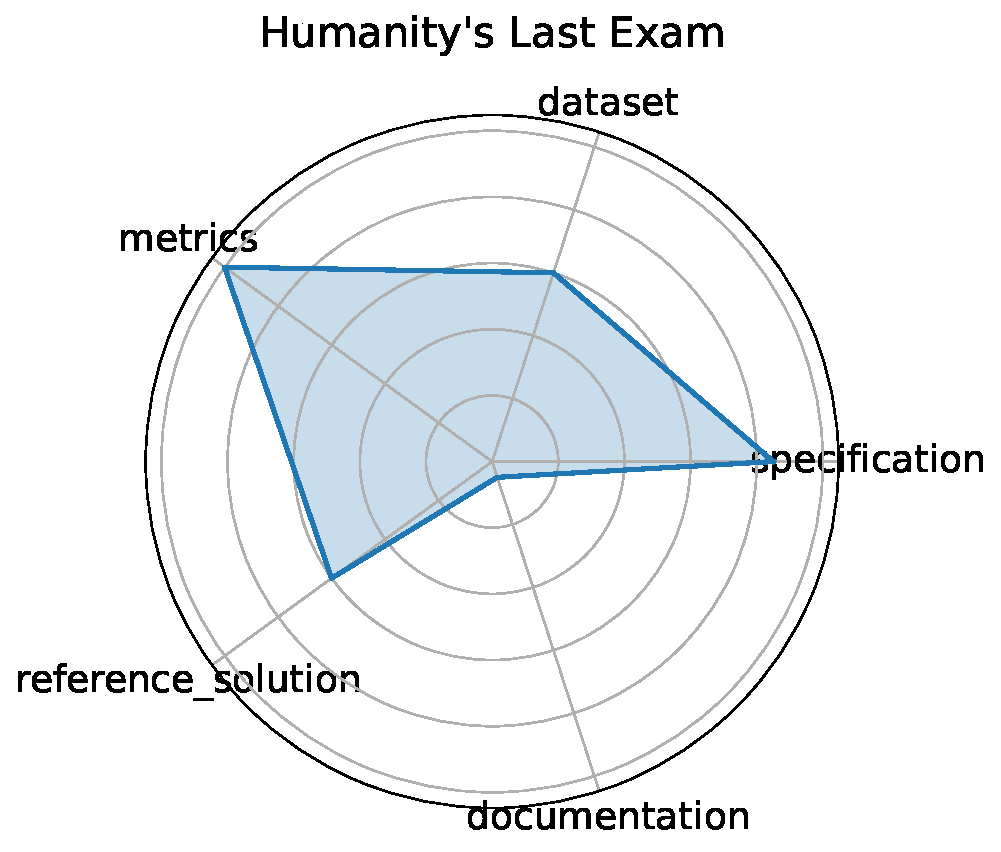
\includegraphics[width=0.2\textwidth]{humanitys_last_exam_radar.pdf}
}}
\clearpage